\chapter{Modelo de Capa Delgada}
\label{chap:hipersonica}

\defcitealias{Canto:1996}{CRW}
\newcommand\CRW{\citetalias{Canto:1996}}

Un ejemplo más realista para la forma de los choques de proa proviene de modelos hidrodinámicos en estado estacionario de la interacción de flujos hipersónicos en el límite de capa delgada. Ejemplos clásicos son la interacción entre dos vientos de \citet{Canto:1996} (\CRW{} de aquí en adelante) y la interacción entre un viento con una corriente plano--paralela \citep{Wilkin:1996}. 
%El problema de interacción de dos vientos es de gran interés en astrofísica, y ha sido estudiado en múltiples ocasiones, principalmente mediante simulaciones hidrodinámicas. Sin embargo, cuando se toman en cuenta diversos factores, incluídos conservación de masa, momento y momento angular, el problema puede resolverse de manera algebraica.
\section{Cantidades conservadas en un flujo hipersónico de capa delgada}

Consideramos dos flujos hipersónicos, no acelerados que forman una capa estacionaria delgada formada por dos choques radiativos separados por una discontinuidad de contacto. El sistema tiene geometría cilíndrica y los vientos no tienen velocidad azimutal. Bajo estos términos, describimos la posición de la capa delgada como $R(\theta)$, donde $R$ es el radio de la capa medido a partir de la posición del origen del viento con menor momento y $\theta$ es el ángulo polar. Asumimos que el gas chocado está bien mezclado, esto implica que  tiene una sola velocidad pos--choque dada por:

\begin{align}
  \vec{v} = v_r \hat{r} + v_z \hat{z}
\end{align}

Donde el eje de simetría del sistema es paralelo a $\hat{z}$, y $\hat{r}$ es el radio cilíndrico. Definimos $\dot{M}(\theta)$, $\vec{\dot{\Pi}}(\theta)$ y $\dot{J}(\theta)$ como la tasa de pérdida de masa, la tasa de momento y la tasa de momento angular, respectivamente, de la capa delgada integradas desde $\theta=0$ hasta $\theta$. Éstas se calculan de la siguiente manera:

\begin{align}
  \vec{\dot{\Pi}}(\theta) &= \dot{\Pi}_r(\theta) \hat{r} + \dot{\Pi}_z(\theta) \hat{z} = \dot{M}\left(v_r \hat{r} + v_z\hat{z}\right) \label{eq:dot-pi}\\
  \vec{\dot{J}}(\theta) &= \vec{R}(\theta) \times \vec{\dot{\Pi}}(\theta)  \\
  \dot{M}(\theta) &= \dot{M}_w(\theta) + \dot{M}_{w1} \label{eq:dot-M}
\end{align}
Donde $\vec{R}(\theta)\equiv R(\theta)\sin\theta~\hat{r} + R(\theta)\cos\theta~\hat{z}$. Resolviendo el producto cruz y tomando su magnitud encontramos que:
\begin{align}
  \dot{J}(\theta) &= \dot{M}(\theta)R(\theta)v_\theta \label{eq:dot-J}\\
  \mathrm{donde:~} & v_\theta = v_r\cos\theta - v_z\sin\theta \label{eq:v-theta}
\end{align}

Por otro lado, al asumir estado estacionario, necesitamos que la tasa de pérdida de masa, la tasa de momento y la tasa de momento angular de la capa delgada sean iguales a aquellas inyectadas por los dos vientos. Entonces definimos estas cantidades como $\dot{M}_w$, $\dot{\Pi}_{wr}$, $\dot{\Pi}_{wz}$ y $\dot{J}_{w}$ para el viento con menor momento, y para el otro viento se utiliza la misma notación solo que utilizando el subíndice ``w1''. De esta forma tenemos que:
\begin{align}
  \dot{\Pi}_r(\theta)\hat{r} + \dot{\Pi}_z(\theta)\hat{z} &= \left[\dot{\Pi}_{wr}(\theta)+ \dot{\Pi}_{wr1}(\theta)\right]\hat{r} + \left[\dot{\Pi}_{wz}(\theta)+ \dot{\Pi}_{wz1}(\theta)\right]\hat{z} \label{eq:Pi-2} \\
  \dot{J} &=\dot{J}_w(\theta) + \dot{J}_{w1}(\theta) \label{eq:J-2}\\
  \dot{M}(\theta) &= \dot{M}_w(\theta) + \dot{M}_{w1}(\theta) \label{eq:M-2}
\end{align}

Combinando las ecuaciones (\ref{eq:dot-pi}, \ref{eq:dot-M}, \ref{eq:dot-J}, \ref{eq:Pi-2}-\ref{eq:M-2}) encontramos que:

\begin{align}
  \dot{M}(\theta)\left[v_r \hat{r} + v_z\hat{z}\right] &= \left(\dot{\Pi}_{wr}(\theta) + \dot{\Pi}_{wr1}(\theta)\right)\hat{r} +
                                                         \left(\dot{\Pi}_{wz}(\theta) + \dot{\Pi}_{wz1}(\theta)\right)\hat{z} \\
  \dot{M}(\theta)v_\theta R(\theta) &= \dot{J}_w(\theta) + \dot{J}_{w1}(\theta)
\end{align}
Y finalmente combinando con la ecuación (\ref{eq:v-theta}) resolvemos para $R(\theta)$:
\begin{align}
  R(\theta) = \frac{\dot{J}_w(\theta) + \dot{J}_{w1}(\theta)}{\left(\dot{\Pi}_{wr}(\theta) + \dot{\Pi}_{wr1}(\theta)\right)\cos\theta - \left(\dot{\Pi}_{wz}(\theta) + \dot{\Pi}_{wz1}(\theta)\right)\sin\theta} \label{eq:R-wind}
\end{align}

\section{Problema de Interacción de Dos Vientos}
\label{sec:CRW-2-winds}
Aplicamos el formalismo ya mencionado para la interacción de dos vientos radiales. El viento con menor momento se localiza en el origen, y su densidad a radio fijo varía con el ángulo polar como una ley de potencias (figura \ref{fig:isotropic-aniso}), o bien, un viento interno con densidad constante e isotrópica:
\begin{align}
  n_{An}(\theta) &=\left\lbrace
  \begin{array}{lr}
    n_0\cos^k\theta  & \mathrm{si~}\theta\leq 90^\circ \\
    0 & \mathrm{si~}\theta > 90^\circ
  \end{array}\right. \label{eq:Ancantoid-density}\\
  n_C &= n_0 \label{eq:cantoid-density}
\end{align}

Donde el índice $k$ indica el grado de anisotropía del viento ``interno''. Cuando la densidad del viento está dada por la ecuación (\ref{eq:cantoid-density}) denominamos a los choques resultantes como ``cantoides'', por \citet{Canto:1996}, mientras que si la densidad está dada por (\ref{eq:Ancantoid-density}) entonces los denominamos ``Ancantoides''. Un caso particularmente interesantes son el viento para un proplyd \citep{HA:1998}, donde $(k=1/2)$. Por el momento restringimos al viento ``externo'' como isotrópico. El problema se muestra de manera esquemática en la figura \ref{fig:crw-esquema}.

Utilizando las ecuaciones (\ref{eq:Ancantoid-density}, \ref{eq:cantoid-density}) encontramos que la tasa de pérdida de masa está dada por:

\begin{align}
  \dot{M}_w = \int^\theta_0\int^{2\pi}_0\rho_w v_w~r^2_0\sin\theta~d\theta~d\phi  \label{eq:general-inner-dot-M}
\end{align}
Donde $v_w$ es la velocidad del viento inteno, $\rho_w = n\bar{m}$  es su densidad, $n$ se obtiene de las ecuaciones (\ref{eq:Ancantoid-density}), $\bar{m}$  es la masa promedio de las partículas del viento y $r_0$ es el radio del viento al cual se alcanza la velocidad terminal $v_w$. Para un proplyd consideramos que dicho radio es el del frente de ionización.

Resolviendo (\ref{eq:general-inner-dot-M}) para vientos con densidades dadas por (\ref{eq:Ancantoid-density}, \ref{eq:cantoid-density}), encontramos que:

\begin{align}
  \dot{M}_w = \dot{M}^0_w\left\lbrace
  \begin{array}{lr}
    \left(1 - \cos^k\theta\right) & \mathrm{Ancantoides} \\
    \frac{1}{2} \left(1 - \cos\theta\right) & \mathrm{Cantoides}
  \end{array}\right. \label{eq:inner-dot-M}
\end{align}
Donde:
\begin{align}
  \dot{M}^0_w = \left\lbrace
  \begin{array}{lr}
    \frac{2\pi}{k+1}\bar{m}n_o v_w r_0^2 & \mathrm{Ancantoides} \\
    4\pi \bar{m}n_o v_w r_0^2 & \mathrm{Cantoides}
  \end{array}\right.
\end{align}

Con esto, obtenemos las tasas de momento y momento angular. Para los choques cantoides, los resultados corresponden a las ecuaciones (9-11) de \CRW{}, sin embargo, para los choques ancantoides, las tasas de momento (axial y radial) y momento angular están dados por:
\begin{align}
  \dot{\Pi}_{wz} &= \int^{\mathrm{min}(\theta, \pi/2)}_0 v_w\cos\theta~d\dot{M}_w = \frac{v_w \dot{M}^0_w}{2\left(k+2\right)}\mathrm{max}\left(1 - \cos^{k+2}\theta, 1\right) \label{eq:Pi-wz} \\
  \dot{\Pi}_{wr} &= \int^{\mathrm{min}(\theta, \pi/2)}_0 v_w\sin\theta~d\dot{M}_w = \frac{1}{2}\dot{M}^0_w v_w I_k(\theta) \\
  \dot{J}_w &= \int^{\mathrm{min}(\theta, \pi/2)}_0 |\vec{R} \times \vec{v}_w|d\dot{M}_w = 0 \label{eq:inner-dot-J}
\end{align}

Donde:
\begin{align}
  I_k(\theta) = \int^{\mathrm{min}(\theta, \pi/2)}_0 \cos^k\theta \sin^2\theta~d\theta \label{eq:Ikt}
\end{align}
 Esta última integral tiene una solución analítica en términos de una función hipergeométrica de la forma ${}_2F_1\left(-\frac{1}{2}; \frac{1+k}{2}; \frac{3+k}{2}; \cos^2\theta\right)$. En el caso particular $k=1/2$, este resultado se ``simplifica'' a una integral de segundo tipo de la forma $E\left(\frac{\theta}{2} | 2\right)$, pero es más sencillo calcularla de manera numérica. La tasa de momento angular para el viento interior es cero debido a que éste se mide respecto al origen, donde se localiza la fuente con menor momento. En este punto los vectores de posición y velocidad para un valor de $\theta$ dado son paralelos.

Para el viento exterior utilizamos las ecuaciones (12-15) y (19-22) de \CRW{} sin cambiar, pero las incluímos en las siguientes secciones por completez.

\subsection{Interacción con un viento esférico isotrópico}
\label{sec:mod-isotropic}

\begin{figure*}
  \begin{tabular}{lr}
    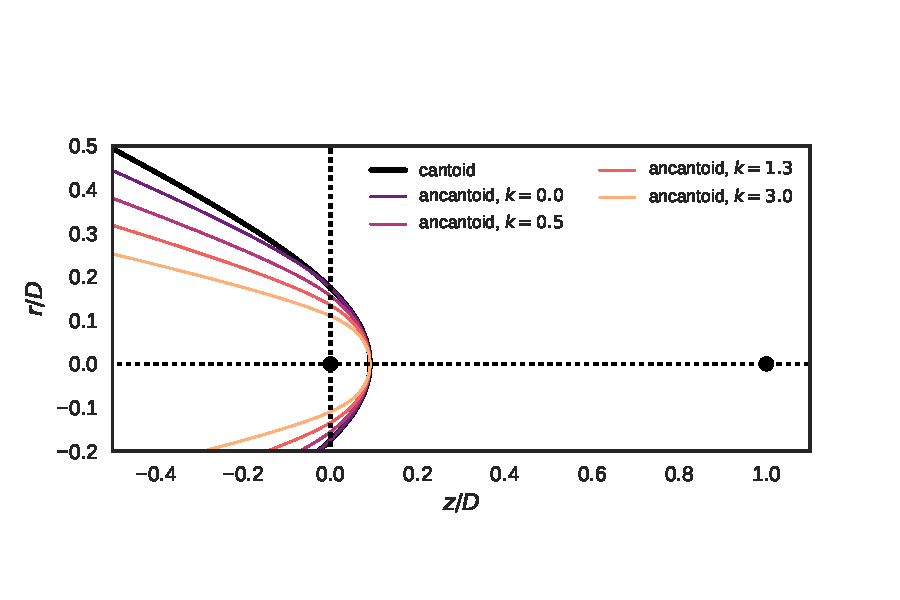
\includegraphics[width = 0.55\linewidth]{./Figures/cantoid-ancantoid-shape-bfixed} &
    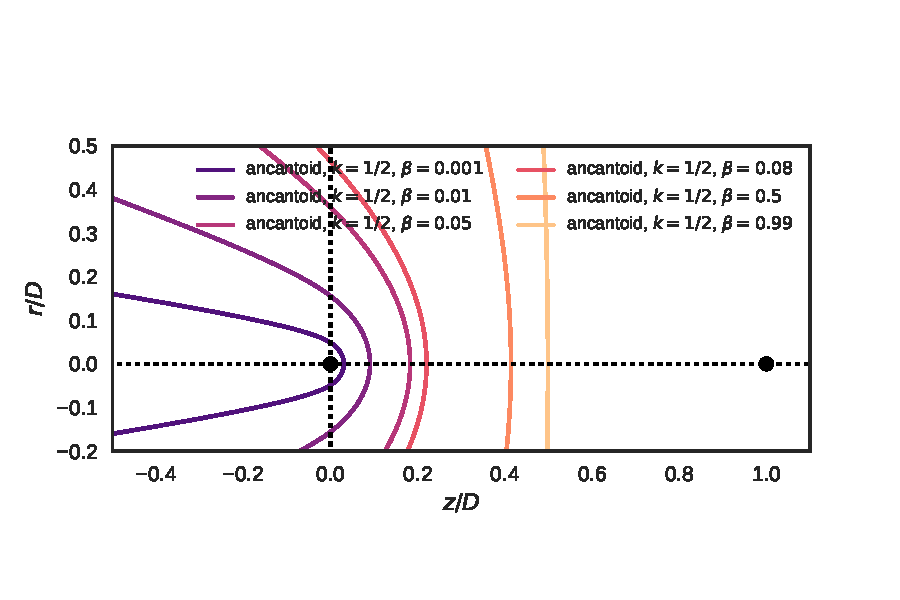
\includegraphics[width=0.55\linewidth]{./Figures/ancantoid-shape}
  \end{tabular}
  \caption{Forma de choques de proa de vientos en interacción. Las coordenadas están normalizadas con $D$, la distancia entre las fuentes de los vientos. La fuente del viento más débil se localiza en el origen $(0, 0)$, mientras que la otra fuente se localiza en $(1, 0)$, ambas marcadas con puntos negros. En (a) los choques de proa mostrados tienen un valor del parámetro $\beta = 0.01$ fijo, mientras que el índice de anisotropía $k$ varía desde 0 hasta 3, mostrados en escala de colores verdes. El choque cantoide con $\beta=0.01$ se muestra en negro. Nótese que el choque ancantoide con $k=0$ es más cerrado en las alas que el tipo cantoide, debido a que en los choques ancantoides la densidad del viento cae a cero cuando $\theta \geq 90^\circ$, mientras que en los cantoides la densidad del viento es constante para toda $\theta$. En (b) el parámetro de anisotropía $k$ es fijo con valor de $1/2$, mientras que el parámetro $\beta$ varía desde $10^{-3}$ hasta $0.99$. La distancia al ápex $R_0$ se incrementa conforme $\beta$ crece, llegando al valor asintótico de $R_0/D = 0.5$ cuando $\beta\to 1$. Lo mismo sucede con el radio de curvatura y $R_{90}$. Algo notable es que en los choques ancantoides aun en el caso límite $\beta=1$, la forma del choque también es curva, debido a que la densidad del viento interior cae con $\theta$ y fuera del eje de simetría el momento del viento exterior es mayor.}
\end{figure}

En este caso tomamos como variable independiente al ángulo polar medido a partir de la posición de la fuente del viento externo, denotado por $\theta_1$. De esta forma las tasas de pérdida de masa, momento y momento angular quedan como sigue:

\begin{align}
  \dot{M}_{w1} &= \frac{M^0_{w1}}{2}\left(1 - \cos\theta_1\right)\\
  \dot{\Pi}_{wz1} &= -\frac{v_{w1}\dot{M}^0_{w1}}{4}\sin^2\theta_1\\
  \dot{\Pi}_{wr1} &= \frac{v_{w1}\dot{M}^0_{w1}}{4}\left(\theta_1 - \sin\theta_1\cos\theta_1\right)\\
  \dot{J}_{w1} &= \int^{\theta_1}_0 R(\theta)v_{w1}\sin(\pi-\theta-\theta_1)~d\dot{M}_{w1} \label{eq:J1}
\end{align}

Utilizando la ley de los senos (ver figura \ref{fig:crw-esquema}), la ecuación (\ref{eq:J1}) queda como sigue:

\begin{align}
  \dot{J}_{w1} &= Dv_{w1}\int^{\theta_1}_0 \sin\theta_1~d\dot{M}_{w1} =
                 \frac{v_{w1}\dot{M}^0_{w1}}{4}\left(\theta_1 - \sin\theta_1\cos\theta_1\right) D \label{eq:J1-iso}
\end{align}

Por otro lado, de la figura \ref{fig:crw-esquema}, podemos deducir la siguiente relación geométrica entre $R(\theta)$,
$\theta$ y $\theta_1$:
\begin{align}
  \frac{R(\theta)}{D} &= \frac{\sin\theta_1}{\sin(\theta+\theta_1)} \label{eq:R-geometric}
\end{align}

Combinando las ecuaciones (\ref{eq:R-wind}, \ref{eq:Pi-wz} - \ref{eq:J1-iso}, \ref{eq:R-geometric}) obtenemos una ecuación implícita que nos indica la dependencia de $\theta_1$ con $\theta$:

\begin{align}
  \theta_1\cot\theta_1 -1 = 2\beta I_k(\theta)\cot\theta - \frac{2\beta}{k+2}\left(1 - \cos^{k+2}\theta\right) \label{eq:th1-th} 
\end{align}
Donde en este caso, la condición de equilibrio de presiones RAM implica que la tasa de momentos $\beta$ ahora está definida como sigue:

\begin{align}
  \beta\dot{M}^0_{w1}v_{w1} = 2(k+1) \dot{M}^0_{w}v_{w}
\end{align}
Sin embargo, (\ref{eq:th1-th}) solo aplica en el rango $0 < \theta \leq \pi/2$. Cuando $\theta > \pi/2$ la relación entre $\theta$ y $\theta_1$ es:

\begin{align}
  \theta_1\cot\theta_1 - 1 = 2\beta\left(I_k(\pi/2)\cot\theta - \frac{1}{k+2}\right) \label{eq:th1-th-far-wings}
\end{align}

Donde:
\begin{align}
I_k(\pi/2) = \frac{\pi}{4}\frac{\Gamma\left(\frac{1+k}{2}\right)}{\Gamma\left(\frac{4+k}{2}\right)} 
\end{align}
y $\Gamma$ es la función Gamma usual.

\subsection{Interacción de un viento esférico isotrópico con un viento plano--paralelo (Choques Wilkinoides)}
\label{sec:wilkinoids}
\begin{figure*} 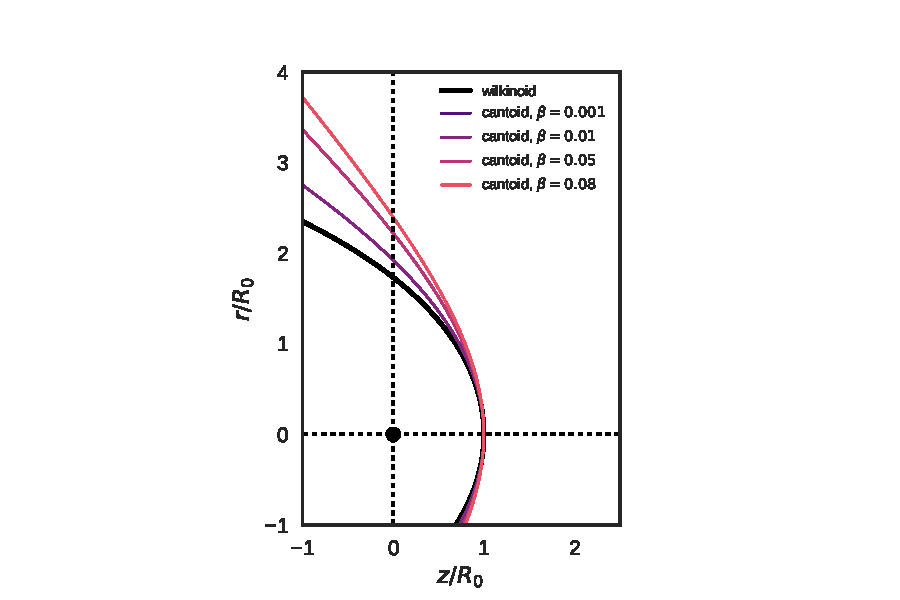
\includegraphics[width=0.6\linewidth]{./Figures/cantoid-wilkinoid-shape}
  \caption{Forma de choques cantoides y el choque wilkinoide. Las coordenadas están normalizadas con la distancia al ápex $R_0$. El choque wilkinoide se muestra en negro y los choques cantoides en escala de azul, con $\beta$ variando desde $10^{-3}$ hasta 0.08. Nótese que el choque wilkinoide se comporta como el caso asíntótico de los choques cantoides cuando $\beta\to 0$.}
\end{figure*}
En este caso las tasas de pérdida de masa, de momento y momento angular del viento plano--paralelo con velocidad $v_a$ y densidad uniforme $\rho_a$ quedan como sigue:
\begin{align}
  \dot{M}_{w1} &= \pi \rho_a v_a R^2 \sin^2\theta\\
  \dot{\Pi}_{wz1} &= - \pi\rho_a v^2_a R^2 \sin^2\theta\\
  \dot{\Pi}_{wr1} &= 0 \\
  \dot{J}_{w1} &= \int^r_0 r'v_a \sin\theta~d\dot{M}_{w1} = \frac{2}{3}\pi\rho_a v_a^2 R^3 \sin^3\theta 
\end{align}
Sustituyendo estas ecuaciones en (\ref{eq:R-wind}) junto con (\ref{eq:inner-dot-M}-\ref{eq:inner-dot-J}) para vientos tipo cantoides $(k=0)$ obtenemos lo siguiente:
\small
\begin{align}
  R = \frac{\frac{2}{3}\pi\rho_a v_a R^3 \sin^3\theta}{\frac{\dot{M}^0_w v_w}{4}\left(\theta-\sin\theta\cos\theta\right)\cos\theta
  - \left(\frac{\dot{M}^0_w v_w}{4}\sin^2\theta - \pi\rho_a v^2_a R^2 \sin^2\theta\right)\sin\theta}
\end{align}
\normalsize
La condición de equilibrio de presión en este caso nos lleva a la siguiente relación:
\begin{align}
  \frac{\dot{M}^0_w v_w}{4\pi R^2_0} = \rho_a v^2_a \label{eq:Wilkin-stagnation}
\end{align}
Por tanto:
\begin{align}
  R/R_0 = \frac{\frac{2}{3}\left(R/R_0\right)^3 \sin^3\theta}{\left(\theta-\sin\theta\cos\theta\right)\cos\theta
  - \left(\sin^2\theta - \left(R/R_0\right)^2 \sin^2\theta\right)\sin\theta}
\end{align}
Resolviendo para $R/R_0$ encontramos que:
\begin{align}
  R = R_0\left[\csc^2\theta\left(1 - \theta\cot\theta\right)\right]^{1/2} \label{eq:R-Wilkin}
\end{align}


\section{Forma ``verdadera'' de los choques cantoides, ancantoides y wilkinoides}

\begin{figure*}
  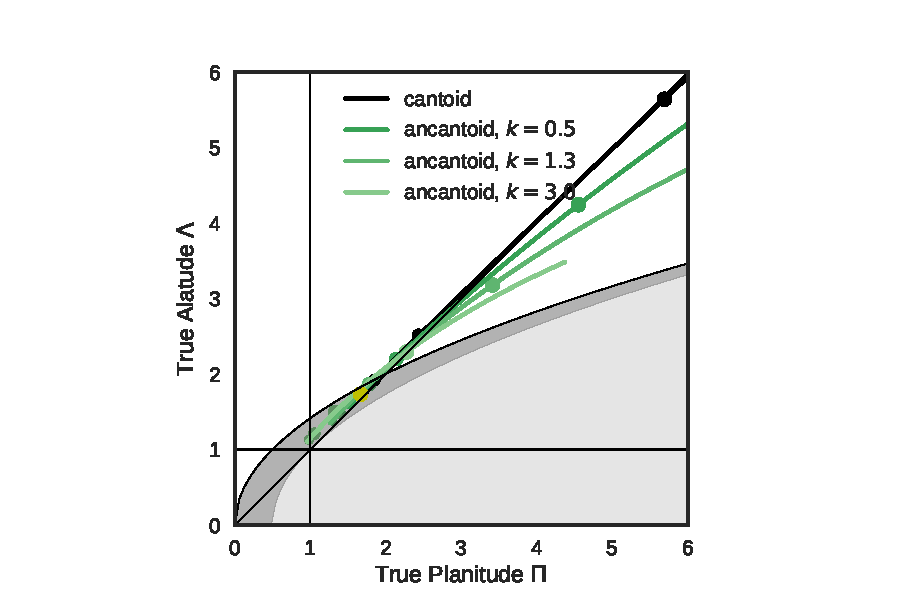
\includegraphics[0.7\linewidth]{./Figures/Pi-vs-Lambda}
  \caption{Forma verdadera de los choques cantoides, ancantoides y wilkinoides. En cada línea, $\beta$ varía en el rango $[0, 1]$, y los parámetros $(\Pi, \Lambda)$ fueron calculados de acuerdo a los resultados del apéndice \ref{app:derivation-radii}. Los círculos del color de las líneas representan valores particulares de $\beta$: $10^{-3}$, $10^{-2}$, 0.1 y 0.5, y con la diferencia de que el coeficiente de segundo orden de la ecuación \ref{eq:CRW-Rc} para la planitud $\Pi$ fue obtenido de manera numérica con el fin de utilizar este método para encontrar la planitud aparente con la ecuación \ref{eq:Rc-prime}}
  \label{fig:true-Pi-Lambda}
\end{figure*}
Para los tres tipos de formas de choques de proa que utilizamos en este trabajo (cantoides, ancantoides y wilkinoides), calculamos su correspondiente alatud y planitud. Para los choques ancantoides obtenemos lo siguiente. El procedimiento detallado se puede consultar en el apéndice \ref{app:derivation-radii}:

\begin{align}
  \Lambda &= \frac{\left(3\xi_k\right)^{1/2}\left(1+\beta^{1/2}\right)} {\left(1+\frac{1}{5}\xi_k\beta\right)^{1/2}\left(1-\xi_k\beta\right)} \label{eq:CRW-R90}\\
  \Pi &= \left|1 - 2\frac{R_{\theta\theta, 0}}{R_0}\right|^{-1} \label{eq:CRW-Rc}\\
  \mathrm{Donde:~} R_{\theta\theta, 0} &= \frac{C_{k\beta}}{1+\beta^{1/2}} + \frac{1 + 2\beta^{1/2}}{3} \label{eq:2-order}
\end{align}
Donde $\xi_k \equiv \frac{2}{k+2}$ y $C_{k\beta}$ son parámetros que se introduce por conveniencia en el apéndice \ref{app:derivation-radii}.

Para los choques cantoides la planitud y alatud son equivalentes al resultado del choque ancantoide con $k=0$, pero se muestran a continuación por completez:

\begin{align}
  \Pi &= \frac{5}{3\left(1-\beta^{1/2}\right)}\label{eq:cantoid-planitude}\\
  \Lambda &= \frac{\sqrt{3}}{\left(1 + \frac{1}{5}\beta\right)^{1/2}\left(1 - \beta^{1/2}\right)} \label{eq:cantoid-alatude}
\end{align}

Por último, el radio en el ápex, la planitud y alatud para los choques wilkiniodes es:

\begin{align}
   R_0 &= \left(\frac{\dot{M}^0_w v_w}{4\pi \rho_a v^2_a}\right)^{1/2} \\
  \Lambda &= \sqrt{3} \label{eq:R90-Wilkin} \\
  \Pi &= \frac{5}{3} \label{eq:Rc-Wilkin}
\end{align}

$R_0$ en este caso se obtiene directamente de la ecuación (\ref{eq:Wilkin-stagnation}), mientras que $\Pi$ y $\Lambda$ se obtienen tomando el límite $\beta\to 0$ en las ecuaciones (\ref{eq:cantoid-planitude}, \ref{eq:cantoid-alatude}), aunque $\Lambda$ también puede obtenerse evaluando la ecuación (\ref{eq:R-Wilkin}) en $\theta=\pi/2$.

En la figura \ref{fig:true-Pi-Lambda} se muestran los resultados de las ecuaciones (\ref{eq:CRW-R90}-\ref{eq:Rc-Wilkin}) en forma de diagrama $\Lambda-\Pi$. Los choques tipo cantoides ocupan en este diagrama una curva, donde cada punto de ésta representa un valor distinto de $\beta$, cuyo rango es $(0, 1)$, y está representada en color negro. Los choques ancantoides ocupan diferentes curvas, una por cada valor del índice de anisotropía $k$, y se representan por curvas con diferente tonalidad de verde, mientras que los choques wilkinoides ocupan un solo punto en este diagrama, representado por el círculo amarillo.

La tendencia general de los choques cantoides y ancantoides es que conforme se incrementan $\beta$ y $k$, también se vuelven más abiertos y más planos en el aṕex ($\Pi$ y $\Lambda$ incrementan), siendo el choque tipo cantoide el más abierto a un valor de $\beta$ dado. Como ya hemos mencionado, el choque tipo cantoide y el tipo ancantoide con $k=0$ son muy similares, excepto que el choque cantoide es más abierto en las alas $(\theta > 90^\circ)$ debido al soporte que da hacia atrás el viento interior. Sin embargo, como su comportamiento es igual para $\theta \leq 90^\circ$, por tanto, no hay diferencia entre estos dos tipos de choques en este diagrama. Todos los choques se encuentran ya sea en la región de esferoides prolatos (región gris oscura) o hiperboloides (región clara), ninguno en la región de esferoides oblatos (ver figura \ref{fig:Pip-Lambdap-diagnostic}a). Los choques tipo esferoide prolato son los que tienen valores de $\beta$ pequeños, y la transición hacia hiperboloide se da cunado $\beta \sim 0.01$ para los choques cantoides y ancantoides con parámetro $k$ pequeño. Esta transición a los hiperboloides se recorre para $\beta$ mayor conforme el parámetro $k$ se incrementa. Esto contrasta con el caso de las cuádricas puras, que siempre permanecen en la misma región, pero esto se debe a que las formas de los choques de proa son más complejas que una cuádrica de revolución: mientras que la forma de la ``cabeza'' del choque (la región cercana al ápex) puede aproximarse bien con una variedad de cuádricas, la forma de las alas lejanas siempre es más parecida a un hiperboloide (ver figura ). El choque wilkinoide se ubica en el límite $\beta\to 0$ de la curva de los choques cantoides, como era de esperarse, y se ubica en la región de esferoides prolatos. Otro detalle que puede apreciarse en esta figura es que todas las curvas (al menos para $\beta$ pequeña) se aglomeran cerca de la diagonal $\Pi \simeq \Lambda$ con la tendencia de que para anisotropía grande, $\Lambda > \Pi$, existe ena región donde hay una degeneración entre $\beta$ y $k$ que se rompe para $\beta$ grande.

Todo esto funciona para la forma verdadera de los choques de proa, que corresponde a cuando son vistos de canto $(i=0)$. La alatud y planitud verdaderas no toman en cuenta el comportamiento de las alas lejanas $(\theta > 90^\circ)$. De hecho, para un choque dado, hay dos formas de calcular el ángulo de las cuádricas $\theta_Q$. Una es a partir de los parámetros $(\Pi, \Lambda)$ utilizando las ecuaciones (\ref{eq:conic-parameter-a-b}, \ref{eq:thc}, \ref{eq:quadric-parameter-pi-lambda}):

\begin{align}
  \theta^{\mathrm{head}}_Q = sgn\left(2\Pi - \Lambda^2\right)~\tan^{-1}\left|2\Pi-\Lambda^2\right|
\end{align}

La segunda manera es a partir de estimar el ángulo asintótico $\theta_\infty$:

\begin{align}
  \theta^{\mathrm{tail}}_Q = \theta_\infty - \pi
\end{align}

Donde $\theta_\infty$ puede obtenerse a partir de la ecuación (28) de \CRW{} para los choques cantoides:

\begin{align}
  \theta_\infty - \tan\theta_\infty = \frac{\pi}{1-\beta}
\end{align}

Mientras que para los choques ancantoides utilizamos la ecuación (\ref{eq:th1-theta-far-wings}) utilizando la condición $\theta_\infty + \theta_{1\infty} = \pi$:

\begin{align}
  \theta_\infty - \left(\frac{k+2(1-\beta)}{k+2}\right)\tan\theta_\infty = \pi + 2\beta I_k(\pi/2)
\end{align}

Como las soluciones a la forma de los choques de proa, tanto cantoides como ancantoides solo ajustan parcialmente a una cuádrica de revolución, entonces $\theta^{\mathrm{head}}_Q \neq \theta^{\mathrm{tail}}_Q$. Esta discrepancia se vuelve relevante al momento de obtener la forma aparente,ya que en este caso la región del choque que es tangente a la línea de visión se aleja del ápex y se acerca a las alas lejanas conforme se incrementa la inclinación.

\section{Obtención de la Forma Aparente}

A continuación aplicamos el formalismo desarrollado en la sección \S \ref{sec:projection} a las formas de los choques de proa obtenidos en este capítulo para obtener tanto la forma aparente como la planitud y alatud aparentes.

En la figura \ref{fig:apparent-cantoid} mostramos la forma aparente de choques tipo cantoides y wilkinoides, y mostramos como referencia un paraboloide confocal cuya forma aparente no cambia con la inclinación (ver \S \ref{sec:pi-lambda-quadric}), mientras que la figura \ref{fig:apparent-ancantoid}} muestra la forma aparente de choques ancantoides.

\begin{figure}
  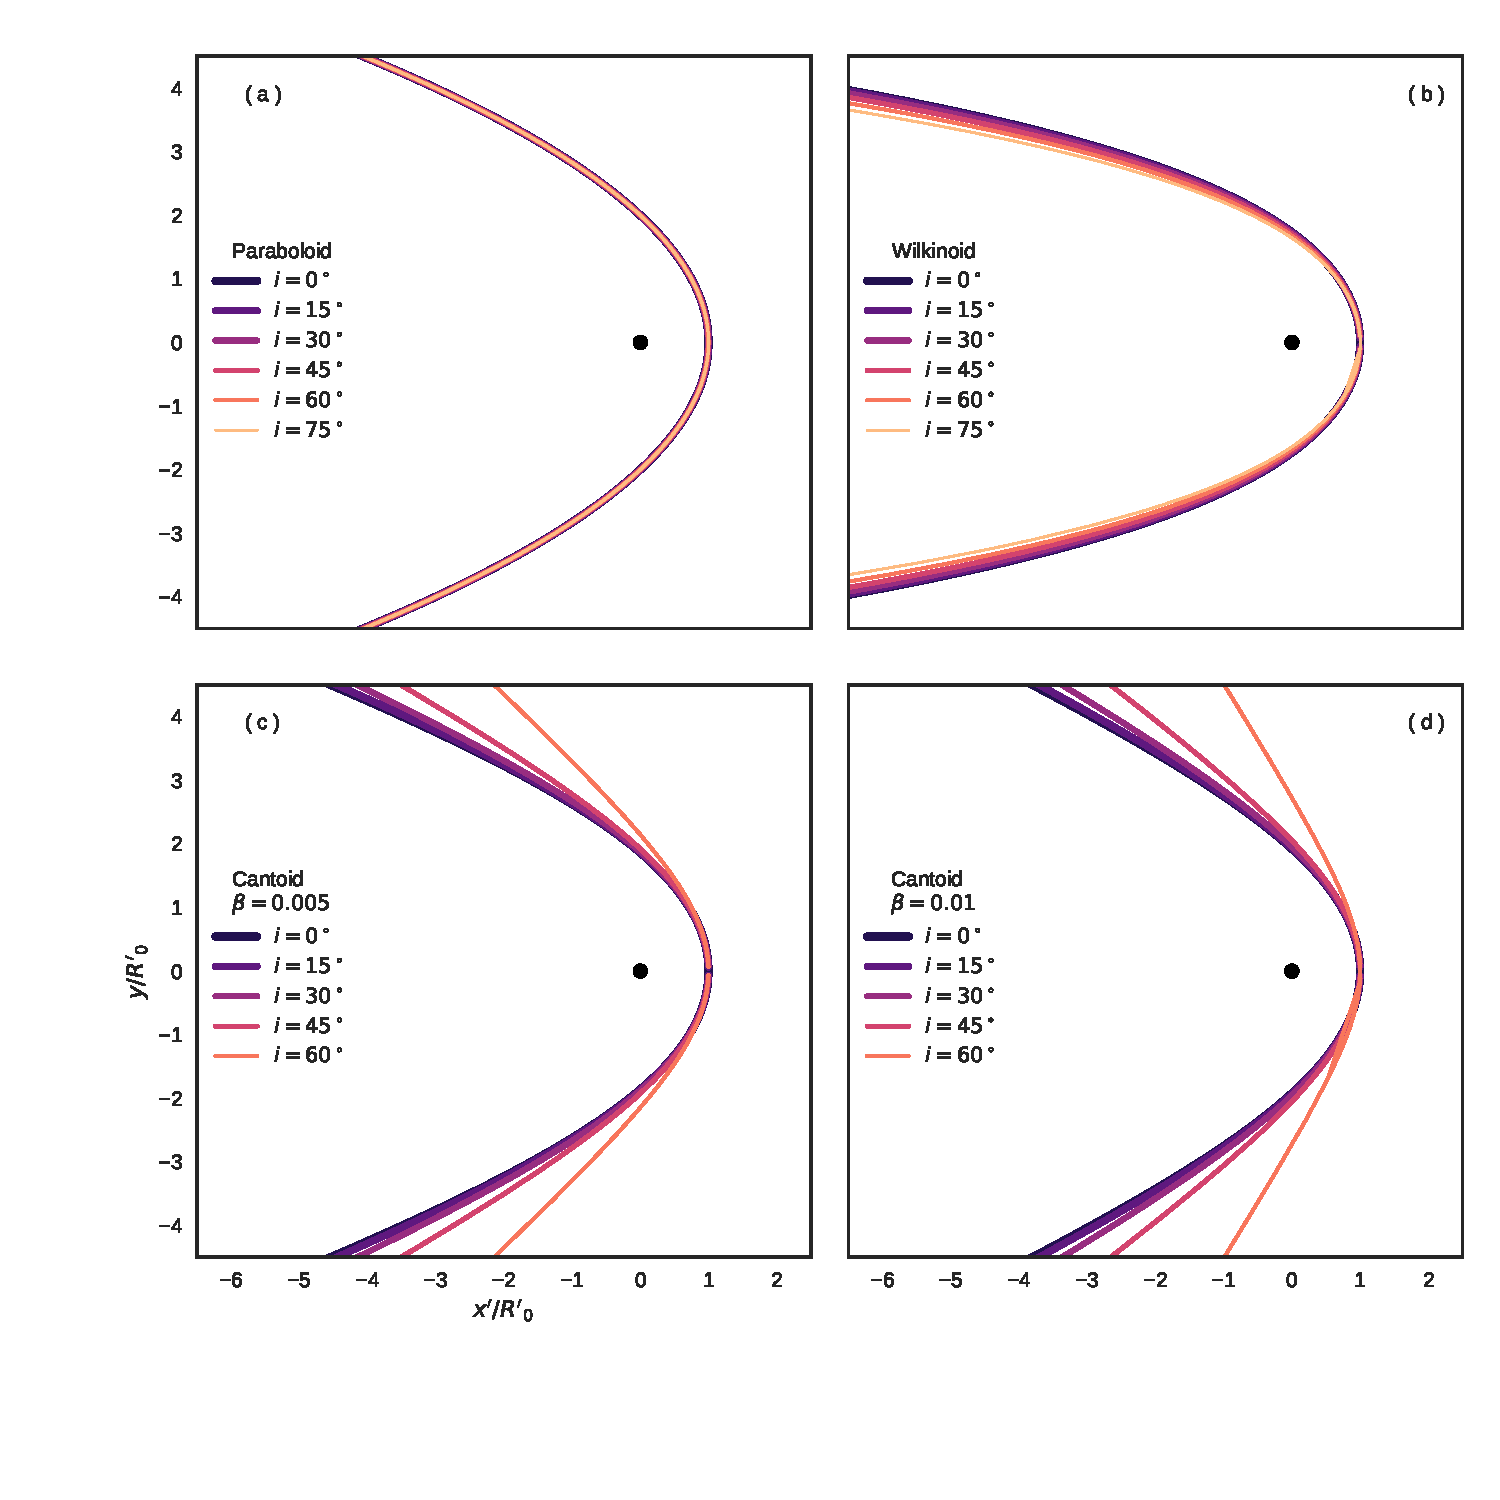
\includegraphics[width=\linewidth]{./Figures/cantoid-apparent-shape}
  \caption{Forma aparente de diferentes choques de proa en intervalos de inclinación de $15^\circ$: (a) Paraboloide confocal. (b) Wilkinoide. (c) Cantoide $\beta=0.005$. (d) Cantoide $\beta=0.01$}
  \label{fig:apparent-cantoid}
\end{figure}

\begin{figure}
  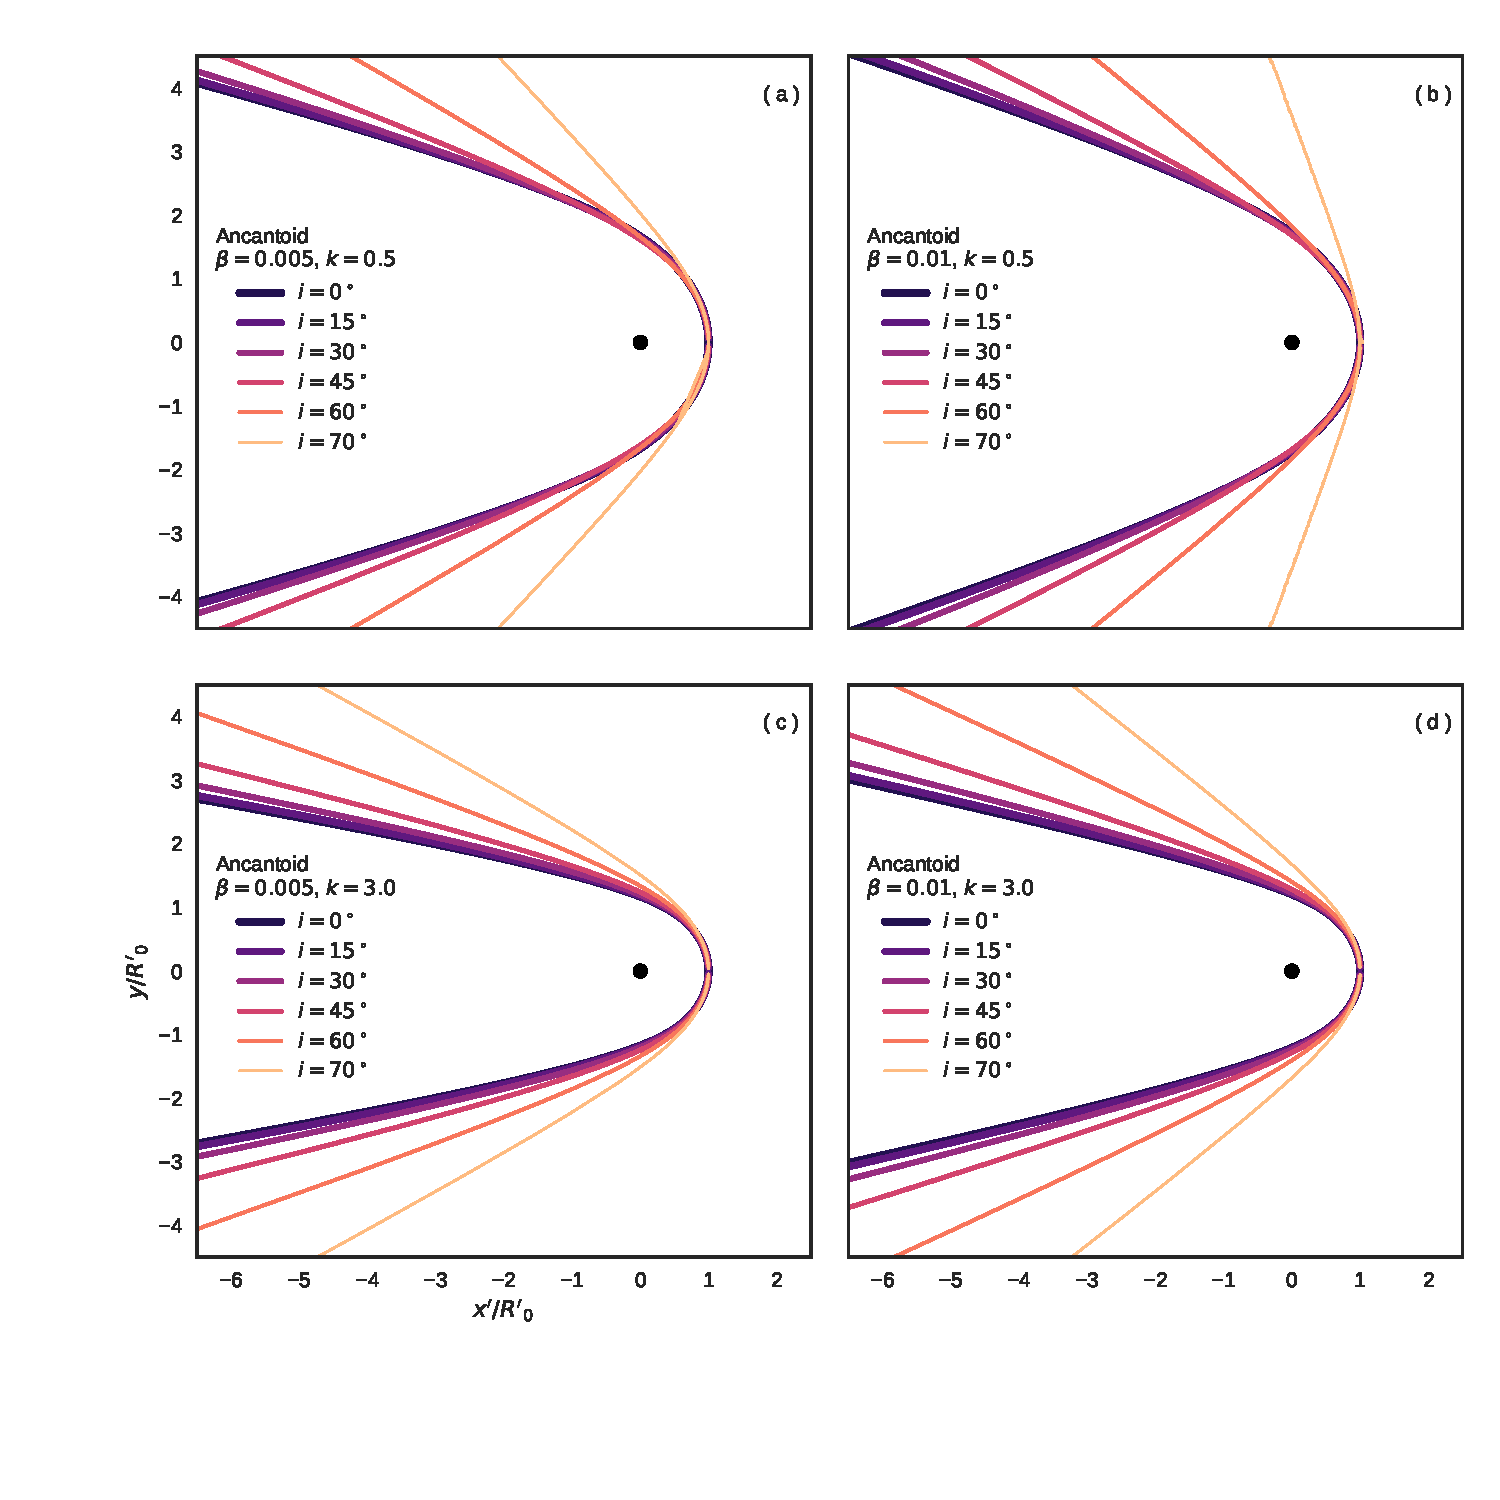
\includegraphics[width=\linewidth]{./Figures/ancantoid-apparent-shape}
  \caption{Extensión de la figura \ref{fig:apparent-cantoid} para choques de proa no isotrópicos (ancantoides): (a) $\beta=0.005$, $k=1/2$. (b) $\beta=0.01$, $k=1/2$. (c) $\beta=0.005$, $k=3$. (d) $\beta=0.01$, $k=3$}
  \label{fig:apparent-ancantoid}
\end{figure}

Se muestra una tendencia general en donde las alas son sistemáticamente más abiertas para altas inclinaciones. Sin embargo, en el caso de los choques Wilkinoides se muestra el comportamiento opuesto, aunque los cambios son muy sutiles. El caso de la figura \ref{fig:apparent-ancantoid}}a, donde se muestra un choque tipo ancantoide con $\beta=0.005$ y $k=1/2$ se observa que para inclinaciones menores a $60^\circ$, las alas cercanas $(\theta\sim 90^\circ)$ se cierran sutilmente, y luego se abren más para inclinaciones mayores.

En la figuras \ref{fig:th0-isotropic} y \ref{fig:th0-anisotropic} mostramos la solución a las ecuaciones (\ref{eq:th-0}, ref{eq:R0p}) para el modelo de capa delgada, junto con el factor de escalamiento $R'_0/R_0$ en función de la inclinación. En estas figuras se observa que el radio aparente en el ápex siempre aumenta con la inclinación, mostrando un crecimiento más rápido para choques más abiertos, pero un incremento mayor para choques más cerrados; ésto debido a que en los choques más cerrados la inclinación máxima donde aun existe una línea tangente es mayor.

\begin{figure}
  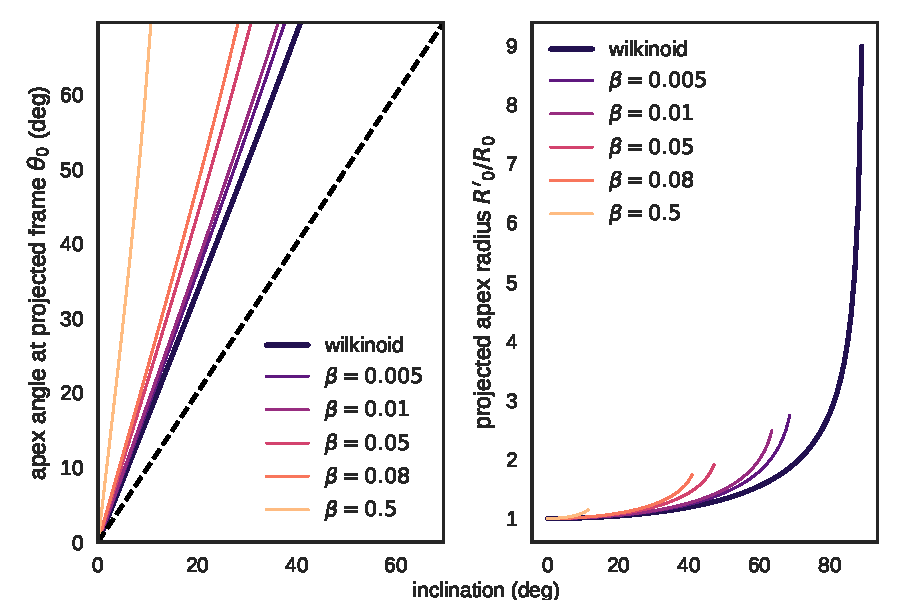
\includegraphics[width=\linewidth]{./Figures/cantoid-th0-vs-i}
  \caption{(a) Soluciones a la ecuación (\ref{eq:th-0}) en función de la inclinación para choques de proa del modelo de capa delgada y viento interior isotrópico (cantoides y wilkinoides). (b) Soluciones a la ecuación (\ref{eq:R0p}) en función de la inclinación normalizadas con $R_0$.}
  \label{fig:th0-isotropic}
\end{figure}

\begin{figure}
  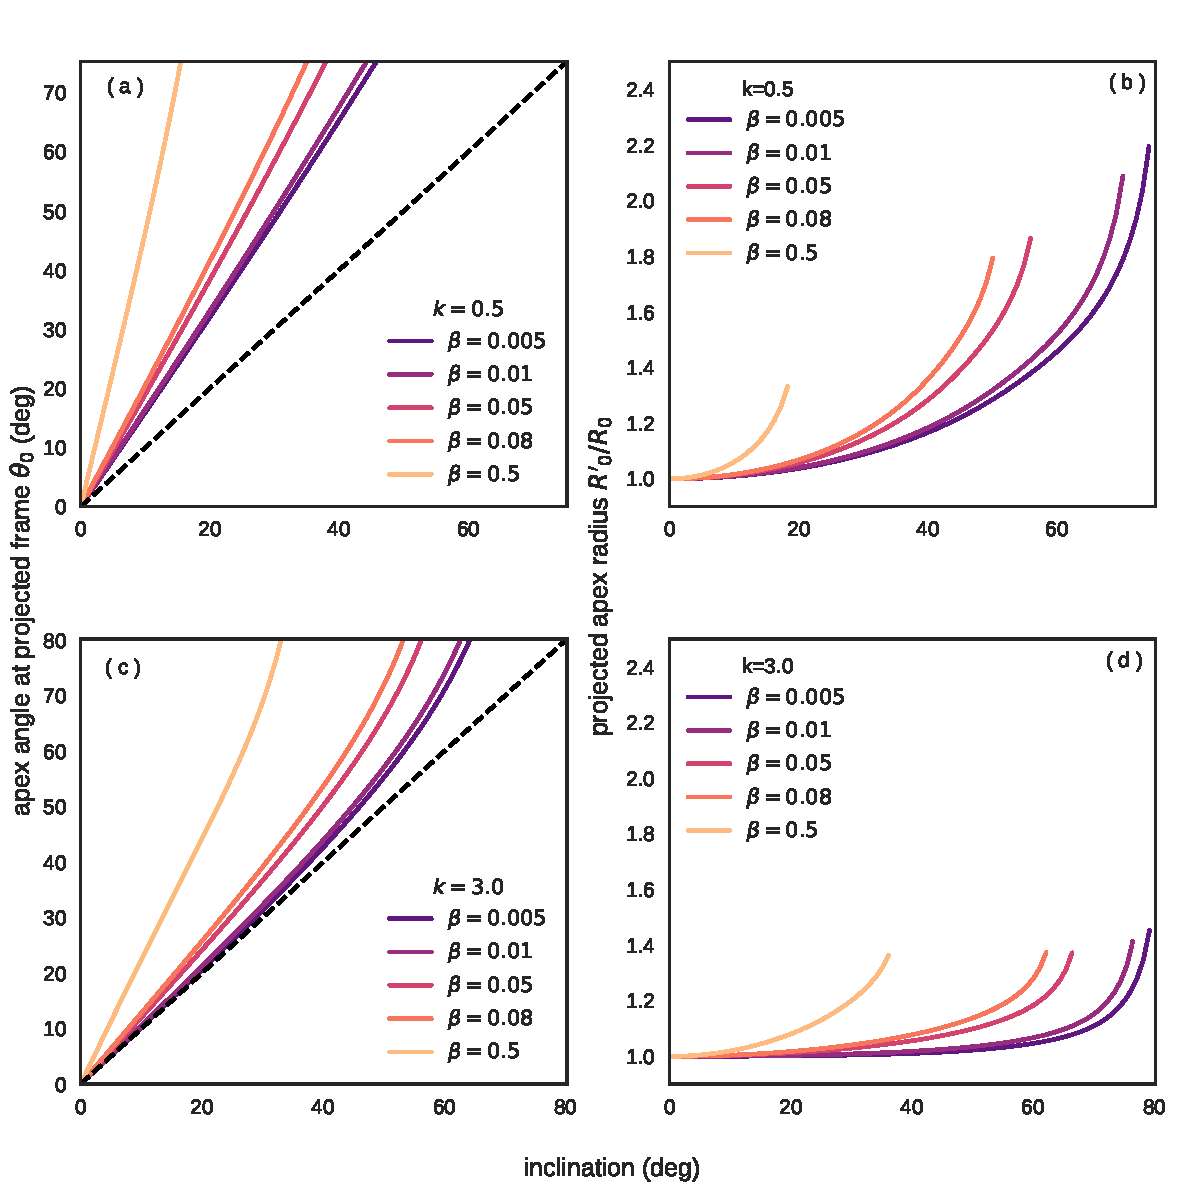
\includegraphics[width=\linewidth]{./Figures/ancantoid-th0-vs-i}
  \caption{(a) Soluciones a la ecuación (\ref{eq:th-0}) en función de la inclinación para choques de proa del modelo de capa delgada y viento interior anisotrópico (ancantoides) para dos índices de anisotropía: $k=1/2$ (arriba) y $k=3$ (abajo). (b) Soluciones a la ecuación (\ref{eq:R0p}) en función de la inclinación normalizadas con $R_0$.}
  \label{fig:th0-anisotropic}
\end{figure}

Las soluciones a las ecuaciones (\ref{eq:th90}, \ref{eq:R90p}) para el modelo de capa delgada se muestran en las figuras \ref{fig:t90-isotropic}, \ref{fig:t90-anisotropic}. Se observa que la alatud aparente se incrementa abruptamente cuando la inclinación se aproxima a la inclinación máxima, excepto en el caso wilkinoide, donde la alatud disminuye con inclinación muy lentamente.

\begin{figure}
  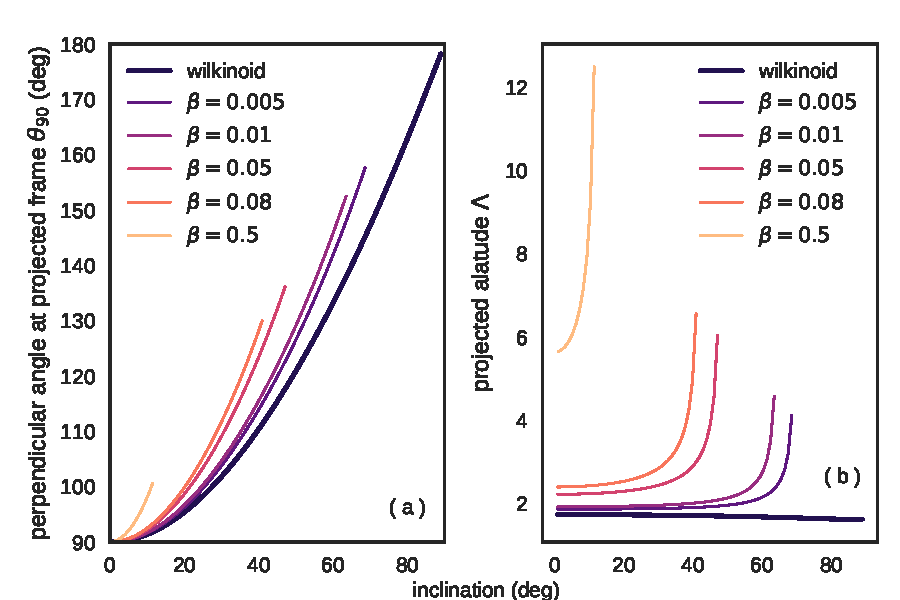
\includegraphics[width=\linewidth]{./Figures/cantoid-th90-vs-i}
  \caption{(a) Soluciones a la ecuación (\ref{eq:th90}) en función de la inclinación para choques de proa del modelo de capa delgada y viento interior isotrópico (cantoides y wilkinoides). (b) Alatud aparente en función de la inclinación, obtenida a a partir del cociente de las soluciones de las ecuaciones (\ref{eq:R90p}, \ref{R0p})}
  \label{fig:t90-isotropic}
\end{figure}

\begin{figure}
  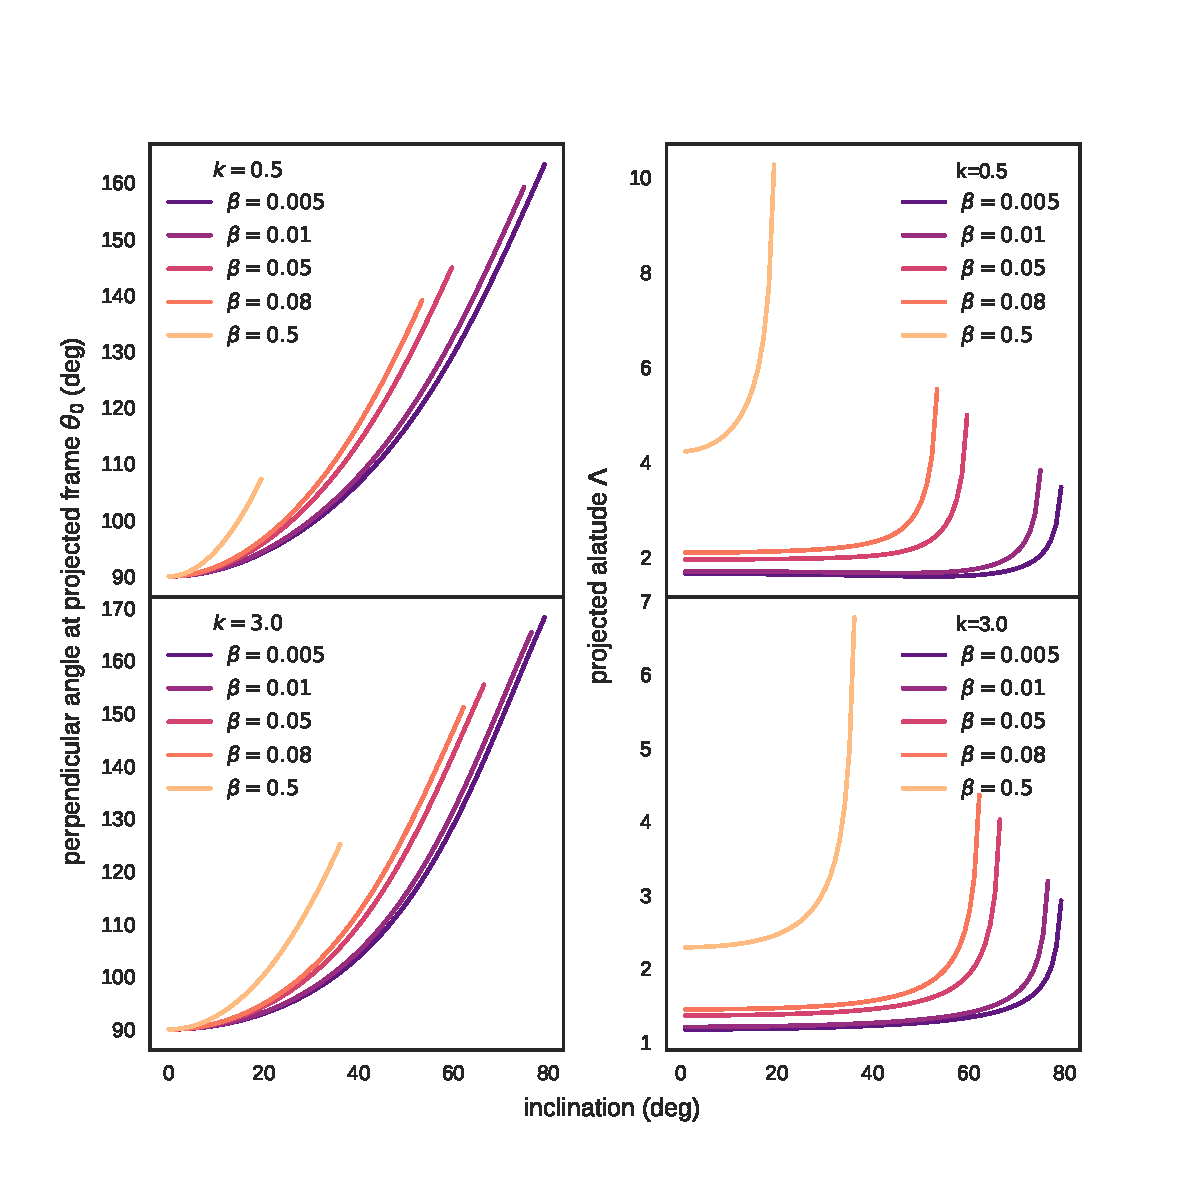
\includegraphics[width=\linewidth]{./Figures/ancantoid-th90-vs-i}
  \caption{(a) Soluciones a la ecuación (\ref{eq:th90}) en función de la inclinación para choques de proa del modelo de capa delgada y viento interior anisotrópico (ancantoides) para dos índices de anisotropía: $k=1/2$ (arriba) y $k=3$ (abajo). (b) Alatud aparente en función de la inclinación, obtenida a a partir del cociente de las soluciones de las ecuaciones (\ref{eq:R90p}, \ref{eq:R0p})}
  \label{fig:t90-anisotropic}
\end{figure}

La planitud aparente se obtuvo a partir de realizar ajustes polinómicos en $\theta^2$ a la forma aparente $R'(\theta')$ para calcular el coeficiente de segundo orden $R'_{\theta'\theta', 0}$ y posteriormente utilizar las ecuaciones (\ref{eq:Rc-prime}, \ref{eq:R0p}). 

Su comportamiento con inclinación se muestra en la figura \ref{fig:Pi-vs-inclination}. Aquí se observa un comportamiento similar al de la alatud aparente; sin embargo, en la figura \ref{fig:Pi-vs-inclination}b, donde el pararámetro de anisotropía es $k=1/2$, se observa una pequeña caída en la planitud justo antes de llegar a la inclinación máxima. 

\begin{figure}
  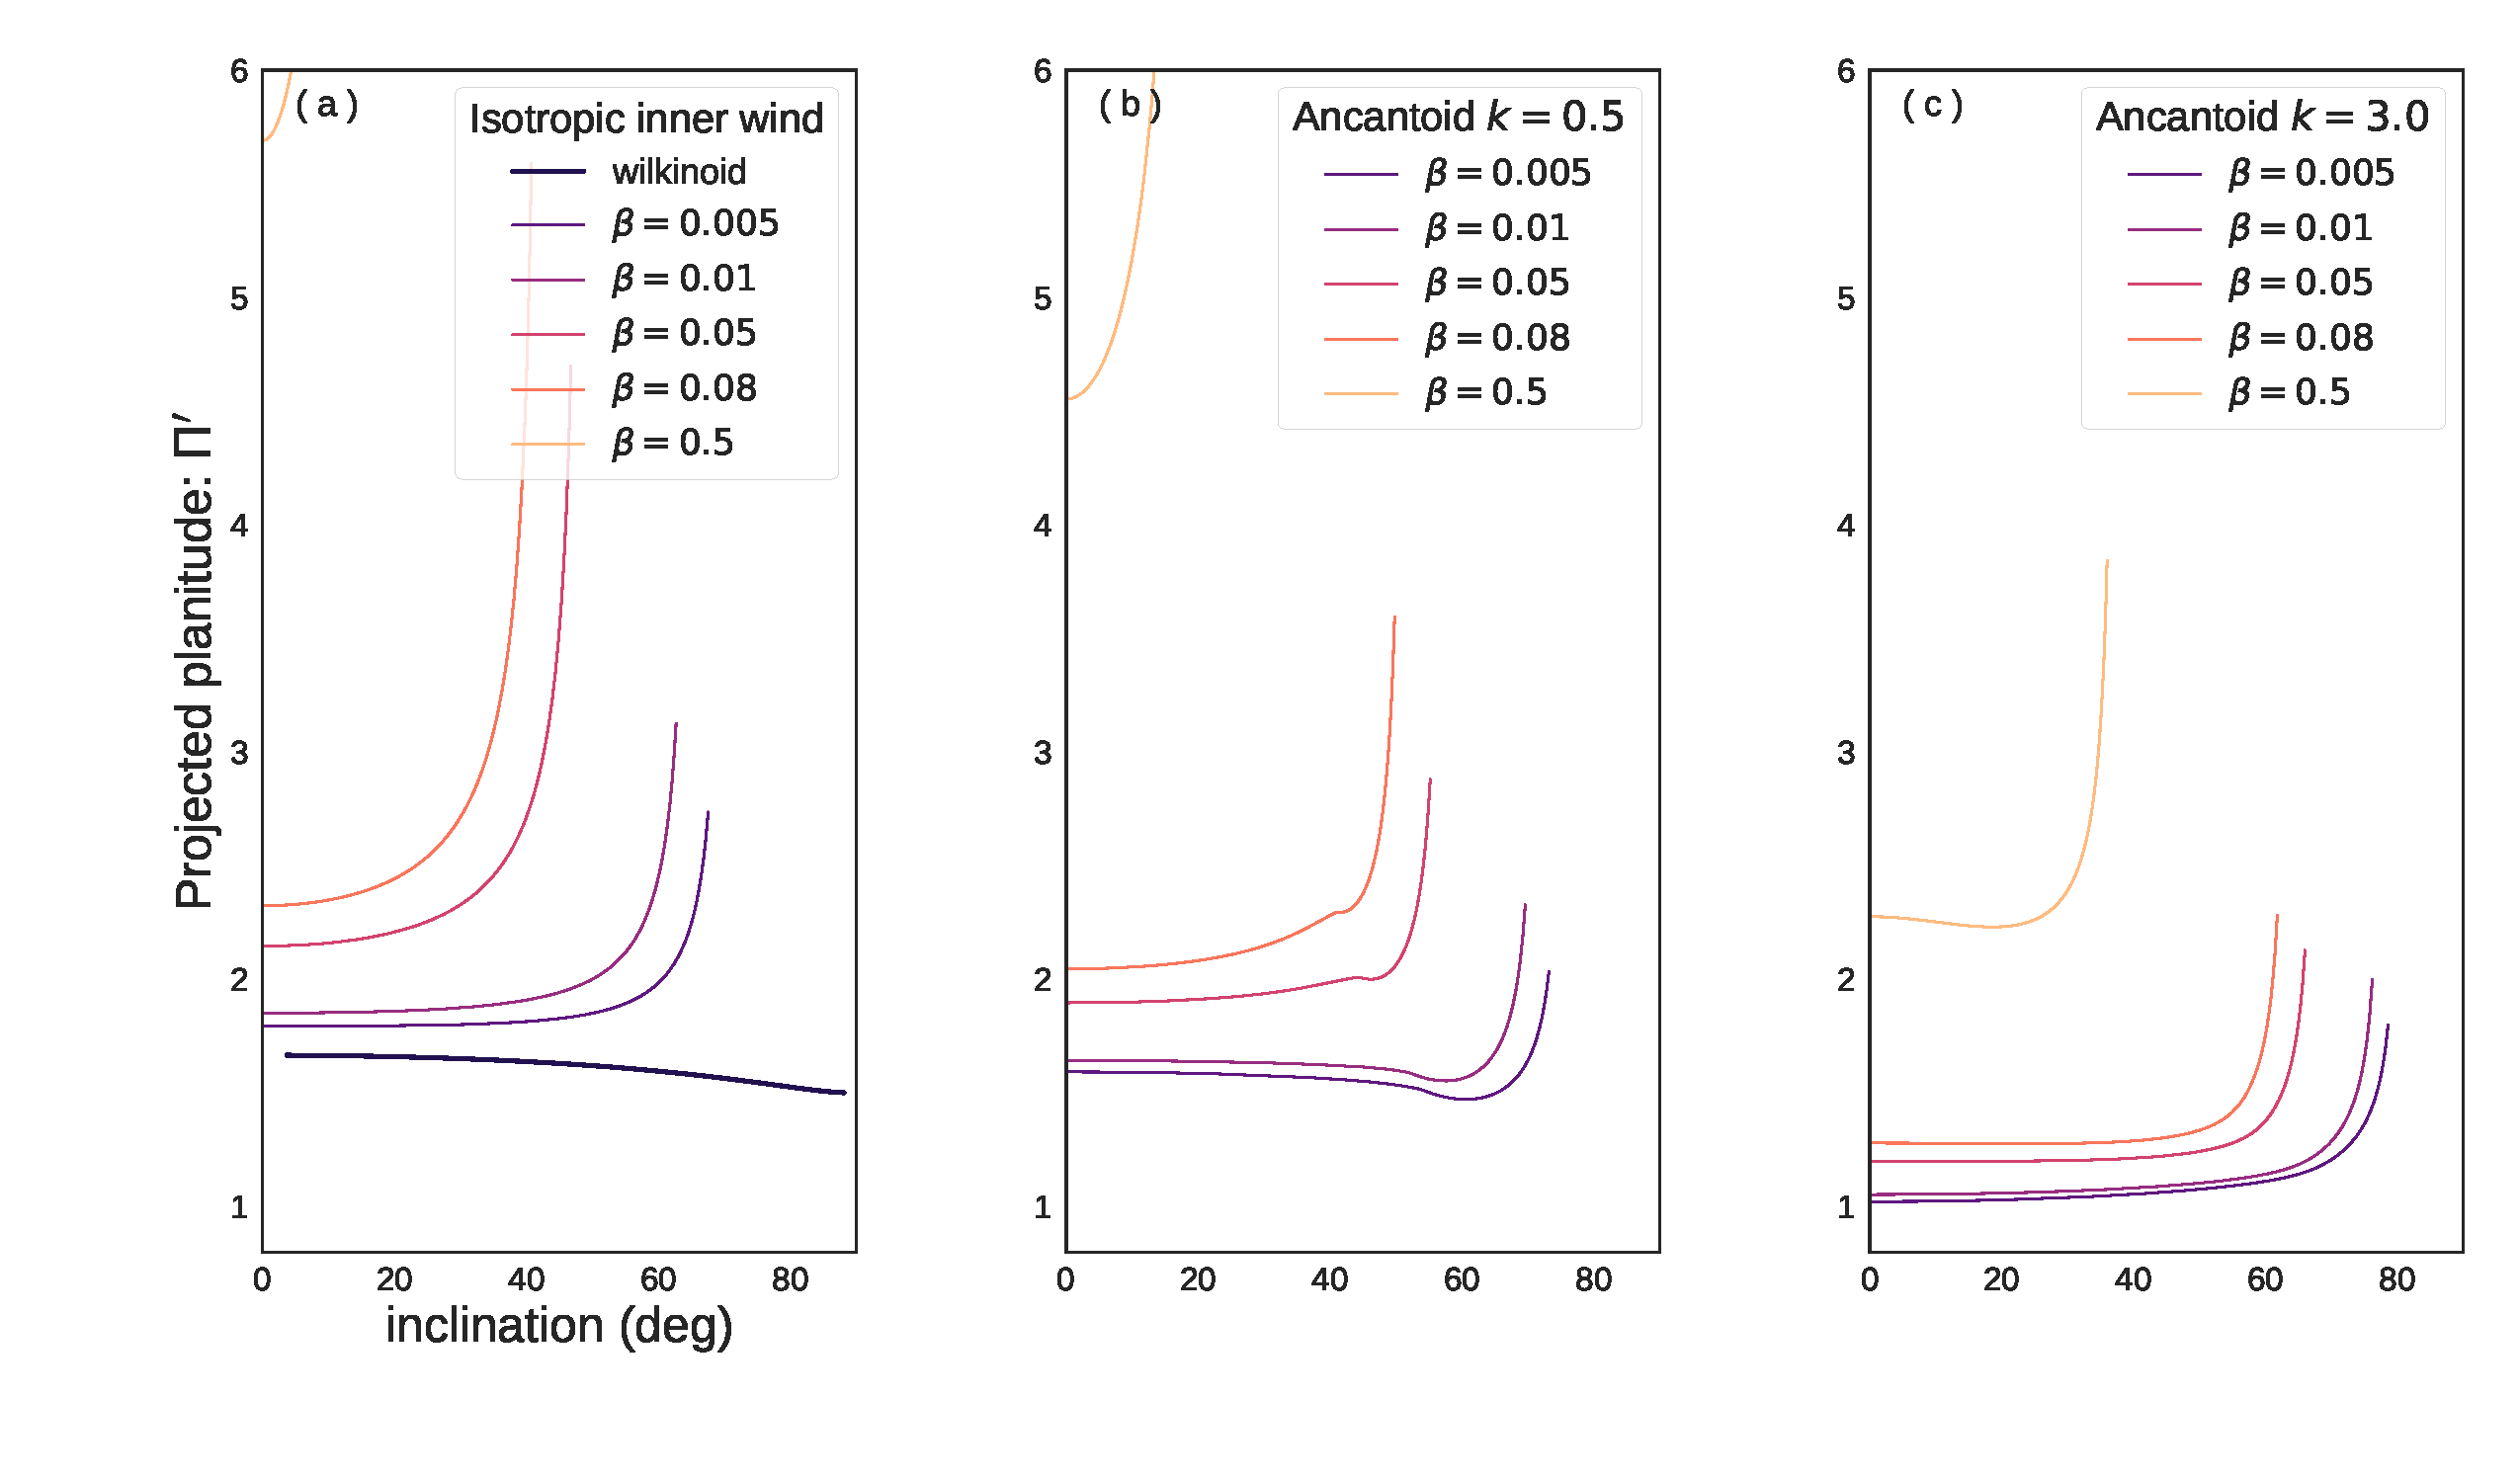
\includegraphics[width=\linewidth]{./Figures/Pi-vs-i}
  \caption{Soluciones a la ecuación \ref{eq:Rc-prime} para obtener la planitud aparente en función de la inclinación en el modelo de capa delgada para: (a) viento interno isotrópico (cantoides y wilkinoides) y viento interno anisotrópico (ancantoides) con índice de anisotropía de (b) $k=1/2$ y (c) $k=3$.}
  \label{fig:Pi-vs-inclination}
\end{figure}

Por último, mostramos en la figura \ref{fig:Lambda-Pi-diagram} los diagramas $\Lambda'-\Pi'$ para diferentes tipos de choques de proa. Cada curva representa un choque de proa con parámetros $(\beta, k)$ fijos donde la inclinación varía de un punto a otro a lo largo de la curva. El comportamiento de estos choques de proa se diferencia del de las cuádricas de revolución, mostrado en la figura \ref{fig:Pip-Lambdap-diagnostic}a. En este caso, las curvas no están confinadas a una sola región: para inclinaciones bajas, la mayoría de las curvas ajustan mejor a la forma de elipsoides prolatos, a excepción de las curvas con parámetro $\beta$ alto $(\beta \gtrsim 0.01)$, mientras que para altas inclinaciones la forma ajusta mejor a hiperboloides. Esto se debe a la tensión que existe entre la forma de la cabeza y de la cola (figura ).

La curva del choque wilkinoide se muestra en color blanco, y tiene un comportamiento menos interesante que otras curvas: simplemente se mueve desde $(5/3, \sqrt{3})$ hasta $(3/2, \sqrt{8/3})$. Aunque se ubica en la región de elipsoide prolato, el hecho de que $\theta_\infty$ sea de $180^\circ$ sugiere que la forma de las alas lejanas sea más parecido al de un paraboloide. Pero converge en $(3/2, \sqrt{8/3})$ en vez de en $(2, 2)$ porque las alas lejanas son asintóticamente cúbicas en vez de cuadráticas.

La densidad de marcas a lo largo de una curva nos indican la probabilidad de observar dicha porción de ésta, si asumimos una distribución isotrópica de ángulos de visión. Se puede observar que la densidad de marcas usualmente se concentra al inicio de cada curva, cerca de $i=0^\circ$, y este efecto se intensifica cuando $\beta$ es pequeño.

\begin{figure}
  \begin{tabular}{lll}
    (a) & (b) & (c) \\
    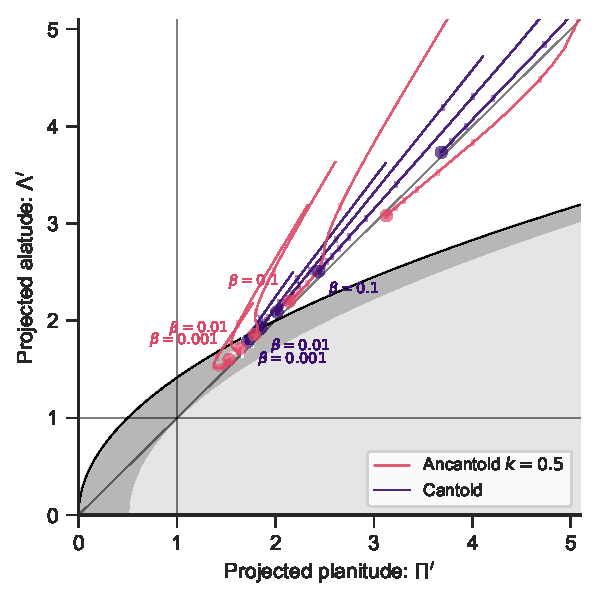
\includegraphics[width=0.33\linewidth]{./Figures/ancantoid-R90-vs-Rc-a} & 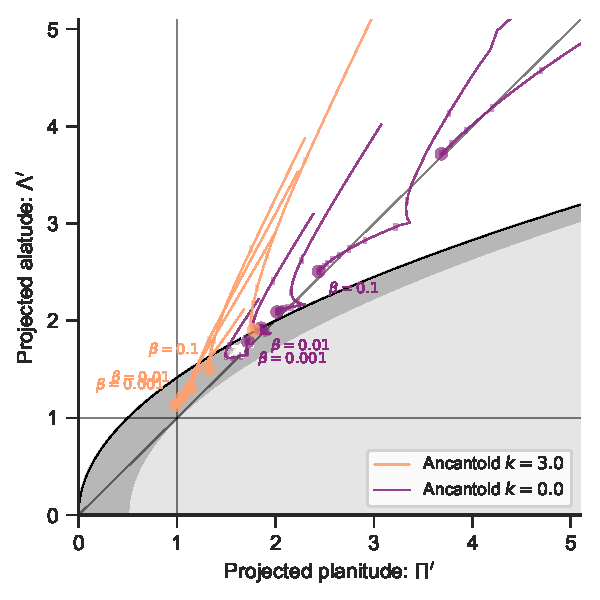
\includegraphics[width=0.33\linewidth]{./Figures/ancantoid-R90-vs-Rc-b}   &                            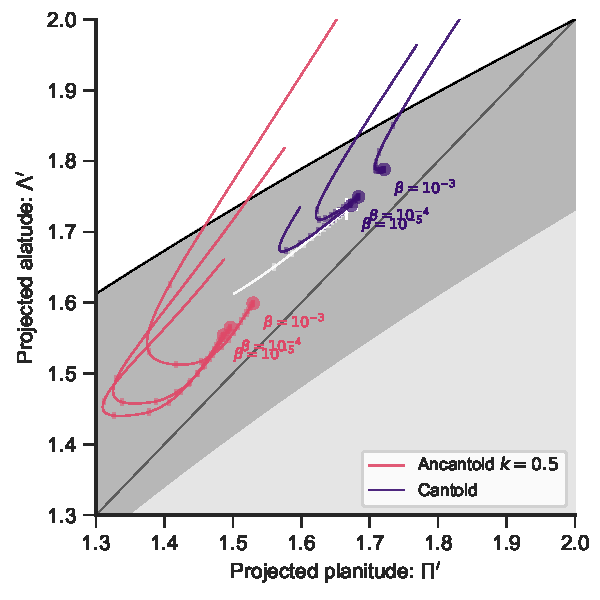
\includegraphics[width=0.33\linewidth]{./Figures/ancantoid-R90-vs-Rc-lobeta-a}                                             
  \end{tabular}
  \caption{Diagramas planitud-ataud para las soluciones del modelo de capa delgada. Los círculos de colores indican la forma intrínseca para cada modelo $(i=0^\circ)$. Las líneas muestran la solución a este mismo modelo en función de la inclinación. Las marcas más pequeñas corresponden a inclinaciones igualmente espaciadas de $|\sin i|$. El modelo wilkinoide se muestra en color blanco. (a) Soluciones para los modelos cantoide (azul) y ancantoide $k=0.5$ (rojo) para $\beta=[0.001, 0.003, 0.01, 0.03, 0.1, 0.3]$. (b) Soluciones para modelos ancantoides $k=3$ (naranja) y $k=0$ (morado). (c) Igual que (a) pero aumentada para mostrar la convergencia de los modelos cantoides hacia el modelo wilkinoide conforme $\beta\to 0$ utilizando como referencia $\beta=[10^{-3}, 10^{-4}, 10^{-5}]$.}
  \label{fig:Lambda-Pi-diagram}
\end{figure}
